\documentclass[compress,red]{beamer}
\mode<presentation>

\usetheme{Warsaw}
\definecolor{Red}{rgb}{1,0,0}
\definecolor{Blue}{rgb}{0,0,1}
\definecolor{Green}{rgb}{0,1,0}
\definecolor{magenta}{rgb}{1,0,.6}
\definecolor{lightblue}{rgb}{0,.5,1}
\definecolor{lightpurple}{rgb}{.6,.4,1}
\definecolor{gold}{rgb}{.6,.5,0}
\definecolor{orange}{rgb}{1,0.4,0}
\definecolor{hotpink}{rgb}{1,0,0.5}
\definecolor{newcolor2}{rgb}{.5,.3,.5}
\definecolor{newcolor}{rgb}{0,.3,1}
\definecolor{newcolor3}{rgb}{1,0,.35}
\definecolor{darkgreen1}{rgb}{0, .35, 0}
\definecolor{darkgreen}{rgb}{0, .6, 0}
\definecolor{darkred}{rgb}{.75,0,0}

\xdefinecolor{olive}{cmyk}{0.64,0,0.95,0.4}
\xdefinecolor{purpleish}{cmyk}{0.75,0.75,0,0}


\useoutertheme[subsection=false]{smoothbars}

\usepackage{multirow}

\usepackage{subfigure}
\usepackage{multicol}
\usepackage{amsmath}
\usepackage{epsfig}
\usepackage{graphicx}
\usepackage[all,knot]{xy}
\xyoption{arc}
\usepackage{url}
\usepackage{multimedia}
\usepackage{hyperref}
\usepackage{setspace}

\title{Inference for the Logconcave NPMLE for Interval Censored Data}
\author{Clifford Anderson-Bergman}
\institute{{\tiny advised by}\\ \vspace{.10cm}Professor Yaming Yu}
\date{\scriptsize Department of Statistics\\ \vspace{.10cm} University of California, Irvine \\ \space{ }}


\begin{document}

\frame{  \titlepage}


\begin{frame}

\frametitle{Interval Censored Data}

	\begin{itemize}

	\item Interval censored data occurs when an event time is known only up to an interval for each subject
	
	\item Define $L_i$ to be the last time known for the event not to have occurred yet occur and $R_i$ to be the first time event is known to have happened
	
		\begin{itemize}
		
		\item Example: subject $i$ has a doctor's visit at $t = 20$ and tests negative for a disease, next visit is at $t = 30$ and tests positive. $L_i = 20$ and $R_i = 30$.
		
		\end{itemize}

	\end{itemize}

\end{frame}

\begin{frame}

\frametitle{Interval Censored Data}

	\begin{itemize}

	\item Case I interval censoring: current status data
	
		\begin{itemize}
		
		\item Subject $i$ is monitored at time $C_i$
			
			\begin{itemize}
			
			\item If event has already occurred, $L_i = 0$ and $R_i = C_i$
			
			\item If event has not occurred, $L_i = C_i$ and $R_i = \infty$
		
			\item All data is either left censored or right censored
			
			\end{itemize}
		
		\item Each observation is very cheap (no need to follow subjects)
		
		\item Each observation is fairly uninformative 
		
		\end{itemize}
	
	\item Case II interval censored data
	
		\begin{itemize}
		
		\item More than one possible observation time (i.e. doctor visits example)
		
		\item Data may be left censored, right censored or within a window
				
		\end{itemize}
	
	\end{itemize}

\end{frame}

\begin{frame}

	\frametitle{Motivating Example}

	\begin{itemize}
	
	\item Study preformed by MacMahon and Worcestor (1966)
	
	\item Outcome of interest: age at menopause
	
	\item Interviewed 2,423 subjects, asked whether they had experienced menopause and if so, when
	
		\begin{itemize}
		
		\item Leads to right censored data
		
		\end{itemize}
	
	\item Researchers noted that there was excessive clustering at digits 0 and 5, likely from recall bias
	
	\item Krailo and Pike (1983) recommended using only menopause status of women at time of the questionnaire
	
	\item Leads to current status data
		
	\end{itemize}

\end{frame}

\begin{frame}

\frametitle{Demand for Non Parametric Estimators for Interval Censored Data}

	\begin{itemize}
	
	\item Non parametric estimators often make fewer assumptions about data structure, reducing potential bias
	
	\item Especially important for interval censored data
	
		\begin{itemize}
		
		\item Typically very difficult to asses model fit: no histograms!
		
		\end{itemize}
	
	\item Downside: reduction in bias often comes with increase in variance
	
	\end{itemize}

\end{frame}

\begin{frame}

\frametitle{Unconstrained NPMLE}

	\begin{itemize}
	
	\item Classic solution: (unconstrained) NPMLE
	
		\begin{itemize}
		
		\item Turbull (1976)
		
		\item Find $\hat F(t) = \underset{F} {\arg \max} \left( \displaystyle \sum_{i = 1}^n \log( F(R_i) - F(L_i) )  \right)$
		
		\item Solution can be written as a discrete probability function
				
		\end{itemize}
	
	\end{itemize}

\centerline{ 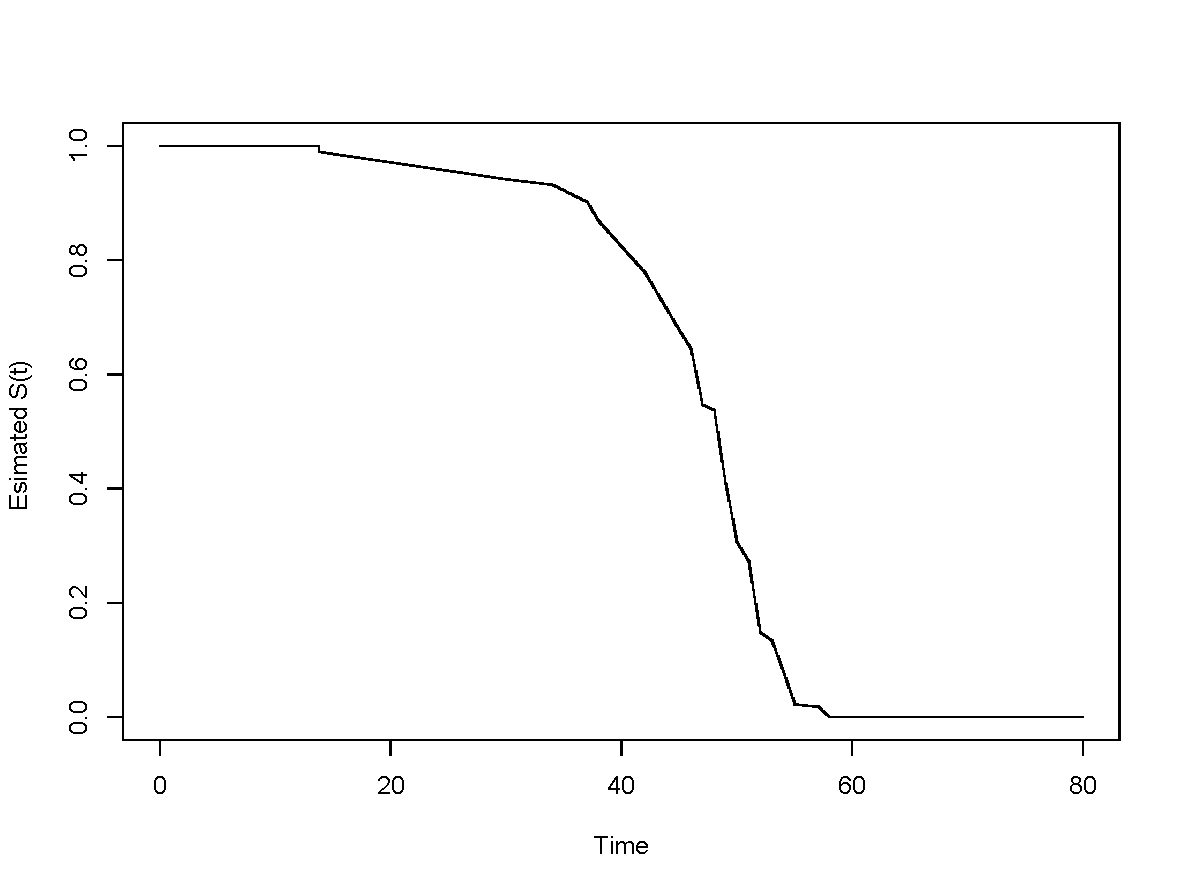
\includegraphics[width = 5cm]{UC_Splot.pdf} }

\end{frame}

\begin{frame}

\frametitle{Issues with Unconstrained NPMLE}

	\begin{itemize}
	
	\item Solution assigns probability mass to isolated intervals
	
		\begin{itemize}
		
		\item Does not dictate how probability mass is assigned within interval
		
		\item No density estimates!
		
		\end{itemize}
		
	\item Solution often jumps erratically, causing excessively high variance of quantile estimates
	
	\item Both problems could be solved by assuming $f_T(t)$ is ``smooth"
	
	\end{itemize}

\end{frame}

\begin{frame}

\frametitle{Modern Non-Parametric Alternatives}

	\begin{itemize}
	
	\item Logspline density estimator (Kooperberg and Stone, 1992)
	
	\item Kernel Smoother (Betensky et al 1999)
	
	\item It has been shown that both these estimators can reduce variance of estimates when compared to unconstrained NPMLE (Pan, W. 2000) 
	
	\end{itemize}

\end{frame}

\begin{frame}

\frametitle{Issues with Modern Non-Parametric Alternatives}

	\begin{itemize}
	
	\item While both estimators work well for light censoring (i.e. narrow intervals), both do poorly under heavy censoring, such as current status data
	
		\begin{itemize}
		
		\item We found kernel smoother often heavily biased
		
		\item Logspline algorithm often gives degenerate estimates or fails!
		
		\item We found these problems to get $worse$ as $n$ increases
		
		\end{itemize}
	
	\end{itemize}

\centerline{ 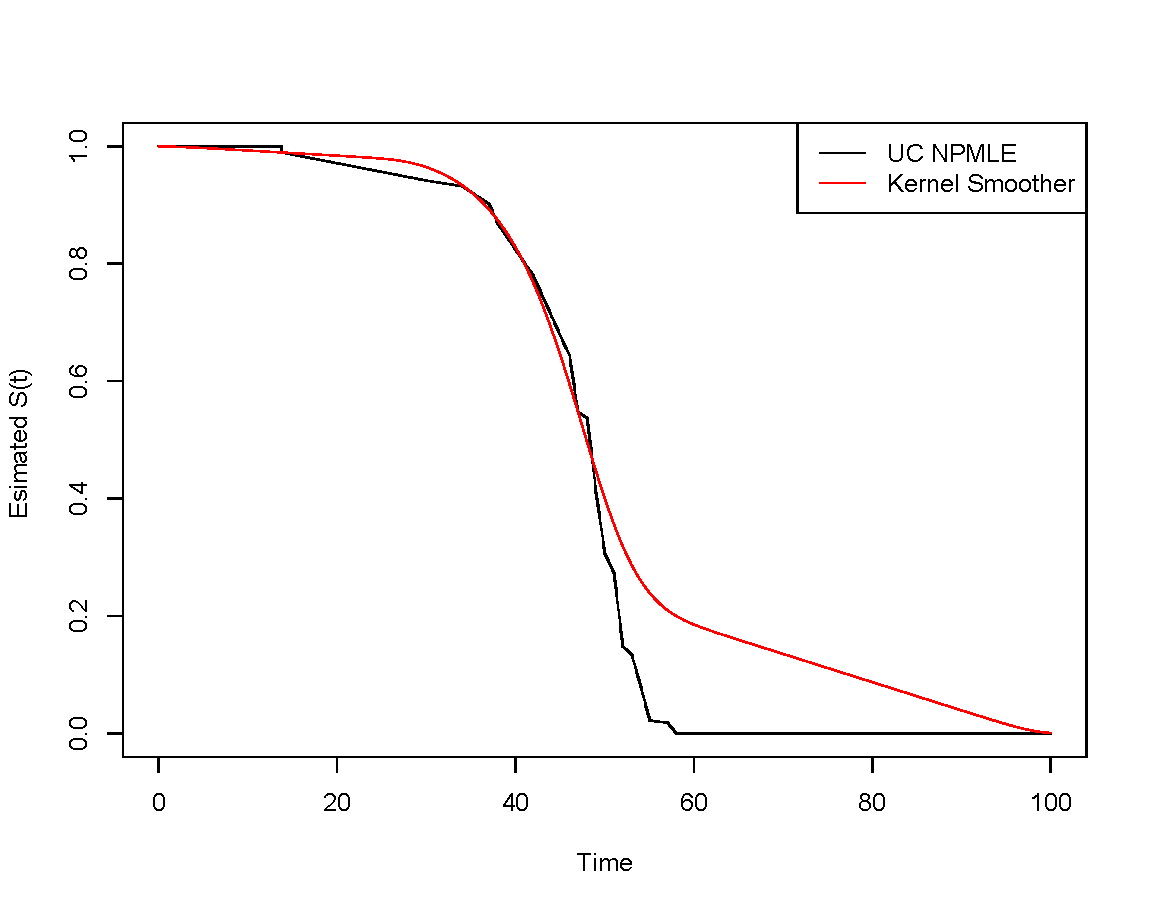
\includegraphics[width = 5cm]{KSplot.pdf} }

\end{frame}

\begin{frame}

\frametitle{Log Concave NPMLE}

	\begin{itemize}
	
	\item We enforce ``smoothness" by assuming logconcavity 
	
		\begin{itemize}
		
		\item $f_T(t) = e^{\phi(t)}$ where $\phi(t)$ is a concave function
		
			\begin{itemize}
			
			\item Insures $f_T(t)$ is unimodal
			
			\item Insures $f_T(t)$ does not have heavier tails than an exponential distribution (exponential distribution is log linear)
			
			\item Insures non-decreasing hazard
			
			\end{itemize}
		
		\item Fairly flexible assumption
		
			\begin{itemize}
			
			\item Normal, gamma with shape $\geq 1$, Weibull with exponent $\geq 1$, beta with both parameters $\geq 1$ and logistic distribution all log concave
			
			\item t, lognormal and multi-modal (common in mixture distributions) are not log concave
			
			\end{itemize}
		
		\end{itemize}
	
	\end{itemize}

\end{frame}


\begin{frame}

\frametitle{Logconcave NPMLE}

	\begin{itemize}
	
	\item D\"umbgen et al (2011) present a very efficient active set algorithm for finding the LC NPMLE with exact observations
		
	\item Chang and Walther (2007) use log concave components for clustering with mixture models
	
	\item D\"umbgen et al (2011) purpose EM algorithm for censored data which discretizes support space, giving approximation of LC NPMLE
	
		\begin{itemize}
		
		\item Current implementation (CRAN package ``logconcens") too slow for moderate sized data sets
		
		\end{itemize}
	
	\end{itemize}

\end{frame}


\begin{frame}

\frametitle{Computing LC NPMLE for Interval Censored Data}

	\begin{itemize}
	
	\item Theorem: an MLE can be achieved via log linear spline with at most $2u-1$ knots, where $u$ = number of unique times in dataset
	
	\item Algorithm: Constructed active set algorithm, similar to D\"umbgen et al 2011, with additional tools to cope with $\ell (\phi)$ not being concave
	
	\end{itemize}

	\begin{table}[H]

\begin{center}	
\caption{Average Computation Times (in seconds)}

\begin{tabular} {| c | c | c | c | c | c | c | c |} 


	 \hline

		 & \multicolumn{7} {|c|} {Unique Times} \\
		
	\hline	
		
	$n$ & 10 & 50 & 100 & 500 & 1000 & 2000 & 5000\\	
		
	 \hline 
 
 	100 & 0.07 & 0.15 & 0.17 & NA & NA &  NA & NA\\ 
	
	\hline
	
	500 & 0.19 & 0.27 & 0.46 & 0.86 & 2.44 & NA & NA\\
	
	\hline
	
	5000 & 0.42 & 0.86 & 1.11 & 5.07 & 7.59 & 31.6 & 156\\ 
	
	\hline
	
\end{tabular}
\end{center}

\end{table}


	
\end{frame}



\begin{frame}

\frametitle{Motivating Example}

	\begin{itemize}
	
	\item LC NPMLE appears to agree with UC NPMLE
	
	\item LC NPMLE solution is once differentialable, UC NPMLE is not 
	
	\end{itemize}

\centerline{ \includegraphics[width = 8.5cm]{Allplot.pdf} }

\end{frame}

\begin{frame}

\frametitle{Simulations}


\begin{table}

\begin{center}
\caption{Quantile Estimation Gamma(100, 2)}

\begin{footnotesize}

\begin{tabular} {| c | c | c | c | c | c | c | } 

	 \hline
	&Q(p)&	43.7 (0.1)&	46.5 (0.25)&	49.8 (0.5)&	53.3 (0.75)&	56.5 (0.9) \\ 
 \hline 
 	n & & \multicolumn{5}{|c|}{Bias / Standard Deviation} 
 \\ 
 \hline 
\multirow{3}{*}{50}		&	LC	&-0.4/2.55	&-0.08/1.54	&-0.05/1.14	&0.06/1.44	&0.72/2.14\\ 
			&	UC	&-0.67/3.73	&-0.23/2.08	&-0.21/1.75	&0.03/2.03	&0.93/2.41\\ 
			&	KS	&11.48/7.22	&3.36/3.15	&-0.1/1.51	&-2.24/1.56	&-3.89/1.92\\ 
	\hline 
\multirow{3}{*}{200}		&	LC	&-0.1/1.13	&0.08/0.73	&-0.02/0.67	&-0.1/0.81	&0.18/1.19\\ 
			&	UC	&-0.17/1.51	&0.04/1.1	&-0.11/1.06	&-0.01/1.23	&0.14/1.82\\ 
			&	KS	&12.64/5.73	&1.88/1.33	&-0.22/0.67	&-1.69/0.93	&-3.83/1.6\\ 
	\hline 
\multirow{3}{*}{800}		&	LC	&0.14/0.68	&0.04/0.44	&-0.07/0.33	&-0.12/0.44	&0/0.61\\ 
			&	UC	&0.1/0.97	&-0.03/0.64	&-0.1/0.51	&-0.05/0.75	&-0.04/0.98\\ 
			&	KS	&15.94/3.23	&1.18/0.66	&-0.25/0.3	&-1.22/0.48	&-4.57/1.35\\ 
	\hline 


\end{tabular}
\end{footnotesize}
\end{center}

\end{table}

\begin{itemize}

	\item SD of LC NPMLE typically about 2/3 SD of UC NPMLE

	\item Kernel smoother does not appear consistent!

\end{itemize}

\end{frame}

\begin{frame}

	\frametitle{Inference for LC NPMLE}
	
	\begin{itemize}
	
	\item Further simulations suggest LC NPMLE is estimator of choice when log concavity assumption is correct
	
	\item Often still best estimator even if mild violations of log concavity 
	
	\item Need some way of evaluating log concavity assumption
	
	\end{itemize}

\end{frame}

\begin{frame}

	\frametitle{Unconstrained Likelihood Ratio Test}

	\begin{itemize}
	
	\item Natural test to consider: Likelihood ratio, comparing LC NPMLE to UC NPMLE
	
	\item Properly nested
	
	\item Problem: very low power!
	
		\begin{itemize}
		
		\item Intuition: UC NPMLE allows for non-log concave and ``unsmooth" estimates
		
		\item Would prefer model which allows for non-log concave but not unsmooth estimates
		
		\end{itemize}
	
	\end{itemize}

\end{frame}

\begin{frame}

	\frametitle{Mixture LC NPMLE}

	\begin{itemize}

	\item After considering several other possible tests, most promising is LR ratio test based on a mixture of 2 LC NPMLE components
	
	\[
	\underset {f_1, f_2, p}{\arg \max} \displaystyle \sum_{i = 1}^n \log( p \int_{L_i}^{R_i} f_1(t) dt + (1-p) \int_{L_i}^{R_i}f_2(t)dt)
	\]
	\[	
	 f_1, f_2 \text{ log concave, } 0 \leq p \leq 1
	 \]

	\item Solution can be found via combination ECM algorithm, using Newton's method to estimate $p$ and earlier algorithm to estimate $f_i$

	\end{itemize}


\end{frame}

\begin{frame}

	\frametitle{Simulations}

	\begin{itemize}
	
	\item Simulations show greater power for mixture LC NPMLE LR test compared to UC NPMLE LR test
	
		\begin{itemize}
		
		\item Strongest gains when distribution really bimodal 
		
		\item Still more powerful if heavily skewed
				
		\item Much more powerful for case II interval censored data than current status data
		
		\end{itemize}
	
	\end{itemize}

\centerline{ \includegraphics[width = 6.5cm]{LRplots.pdf} }

\end{frame}


\begin{frame}

\frametitle{Future Work: Difficulties in Implementing Test}

	\begin{itemize}

	\item The family of single component LC distributions are on the boundary of 2 component LC mixture distributions
	
	\item Typically it is suggested to sample under the null hypothesis to find p-value
	
	\item Problem: Censoring distribution affects likelihood!
	
		\begin{itemize}
		
		\item For current status data, very easy to model censoring distribution
		
		\item For general case II interval censoring, much more difficult...
		
		\end{itemize}

	\end{itemize}

\end{frame}

\begin{frame}

\frametitle{Future Work: Computational Issues}

	\begin{itemize}
	
	\item Mixture models are known to have several local maximum points, making finding the true MLE difficult
	
	\item Random starting points in our algorithm demonstrates this can be a problem for the mixture LC NPMLE
	
		\begin{itemize}
		
		\item Differences in likelihoods occasionally observed to be higher than 1.0!
		
		\item Fixing this may increase power of test
		
		\end{itemize}
		
	\item Try applying methods used for general mixture models to efficiently deal with this
	
	\end{itemize}

\end{frame}

\end{document}